\chapter{Johdanto}

Kurssin \emph{Tietorakenteet ja algoritmit} tarkoituksena
on opettaa menetelmiä, joiden avulla voimme ratkaista
\emph{tehokkaasti} laskennallisia ongelmia.
Ohjelmoinnin peruskursseilla olemme keskittyneet
ohjelmointitaidon opetteluun.
Nyt on aika siirtyä askel eteenpäin ja alkaa kiinnittää
huomiota myös siihen, miten nopeasti algoritmit toimivat.

Algoritmien tehokkuudella on suuri merkitys käytännössä.
Esimerkiksi netissä toimiva reittiopas on käyttökelpoinen sen vuoksi,
että se antaa meille reitin kuvauksen heti sen jälkeen, kun olemme
ilmoittaneet, mistä mihin haluamme matkustaa.
Jos meidän pitäisi odottaa reitin kuvausta vaikkapa minuutti tai tunti,
tämä rajoittaisi paljon palvelun käyttöä.

Jotta reittiopas toimisi tehokkaasti, sen taustalla on
hyvin suunniteltu algoritmi.
Tällä kurssilla opimme, kuinka voimme luoda itse vastaavia algoritmeja.
Tutustumme kurssilla sekä algoritmien suunnittelun teoriaan että
käytäntöön -- haluamme ymmärtää syvällisesti, mistä algoritmeissa on kysymys,
mutta myös osata toteuttaa niitä käytännössä.

\section{Mitä algoritmit ovat?}

Algoritmi on toimintaohje, jota seuraamalla voimme ratkaista
jonkin laskennallisen ongelman.
Algoritmille annetaan \emph{syöte},
joka kuvaa ratkaistavan ongelman tapauksen,
ja algoritmin tulee tuottaa \emph{tuloste},
joka on vastaus sille annettuun syötteeseen.

Tarkastellaan esimerkkinä laskennallista ongelmaa,
jossa syötteenä on $n$ kokonaislukua ja haluttu
tuloste on lukujen summa.
Esimerkiksi jos syöte on $[2,4,1,8]$,
haluttu tuloste on 15, koska $2+4+1+8=15$.
Voimme ratkaista tämän ongelman algoritmilla,
joka käy luvut läpi silmukalla ja laskee niiden
summan muuttujaan.

Algoritmin toiminnan esittämiseen on useita mahdollisuuksia.
Yksi tapa on selostaa sanallisesti, kuinka algoritmi toimii,
kuten teimme äsken.
Toinen tapa taas on antaa koodi, joka toteuttaa algoritmin.
Tällöin meidän täytyy valita jokin ohjelmointikieli,
jonka avulla esitämme algoritmin.
Esimerkiksi seuraava Java-koodi kuvaa algoritmin,
joka laskee lukujen summan:

\begin{code}
int summa = 0;
for (int i = 0; i < n; i++) {
    summa += luvut[i];
}
System.out.println(summa);
\end{code}

Voimme myös esittää algoritmin \emph{pseudokoodina}
todellisen ohjelmointikielen sijasta.
Tämä tarkoittaa, että kirjoitamme koodia,
joka on lähellä käytössä olevia ohjelmointikieliä, mutta voimme
päättää koodin tarkan syntaksin itse ja ottaa joitakin vapauksia,
joiden ansiosta voimme kuvata algoritmin mukavammin.
Voisimme esimerkiksi esittää äskeisen algoritmin pseudokoodina seuraavasti:

\begin{code}
summa = 0
for i = 0 to n-1
    summa += luvut[i]
print(summa)
\end{code}

Tässä kirjassa esitämme algoritmeja sekä Java-koodina että pseudokoodina
tilanteesta riippuen.
Käytämme Java-koodia silloin, kun haluamme erityisesti kiinnittää huomiota siihen,
miten jokin asia toteutetaan käytännössä Javassa.
Pseudokoodia käytämme taas silloin, kun haluamme kuvata algoritmin yleisen
idean eikä käytetyllä kielellä ole merkitystä.

\section{Ohjelmoinnin peruspalikat}

Kiehtova seikka ohjelmoinnissa on, että monimutkaisetkin algoritmit
syntyvät yksinkertaisista aineksista.
Käymme seuraavaksi läpi ohjelmoinnin peruspalikat,
jotka muodostavat pohjan algoritmien suunnittelulle.

\subsubsection{Muuttuja}

Muuttujat säilyttävät algoritmissa tarvittavia tietoja.
Useimmissa algoritmeissa muuttujissa on kokonaislukuja.

\begin{code}
a = 1
b = 2*a+3
\end{code}

\subsubsection{Ehtolause}

Ehtolauseen avulla saamme ohjelman toiminnan
riippumaan muuttujista.
Esimerkiksi seuraava koodi kertoo, onko $x$ parillinen vai pariton:

\begin{code}
if x%2 == 0
    print("parillinen")
else
    print("pariton")
\end{code}

\subsubsection{Silmukka}

Silmukoiden avulla voimme toistaa koodia.
Seuraava for-silmukka tulostaa luvut $1 \dots 10$:

\begin{code}
for i = 1 to 10
    print(i)
\end{code}

Seuraava while-silmukka puolestaan puolittaa lukua $x$,
kunnes se saavuttaa nollan:

\begin{code}
while x > 0
    print(x)
    x /= 2
\end{code}

\subsubsection{Taulukko}

Taulukko on ohjelmoinnin tavallisin \emph{tietorakenne}
eli tapa säilyttää kokoelmaa tietoa.
Taulukossa on $n$ alkiota, joiden kohdat ovat $0,1,\dots,n-1$.

\begin{code}
x = [4,2,7,5,1]
print(x[2]) // 7
x[2] = 3
print(x[2]) // 3
\end{code}

Tutustumme kirjan aikana moniin tietorakenteisiin,
joista on hyötyä algoritmien suunnittelussa.
Kaikki tietorakenteet perustuvat kuitenkin pohjimmiltaan taulukkoon.

\subsubsection{Funktio}

Funktioiden avulla voimme jakaa koodia osiin.
Javassa funktioita kutsutaan yleensä metodeiksi.

\begin{code}
function summa(a,b)
    return a+b
\end{code}

\subsubsection{***}

Olemme nyt käyneet läpi ainekset,
joiden avulla voimme toteuttaa \emph{minkä tahansa} algoritmin.
On huojentava tieto, että näinkin pieni määrä tekniikoita
riittää algoritmien suunnittelussa.
Nyt kaikki on vain kiinni siitä, miten osaamme \emph{soveltaa}
näitä tekniikoita eri tilanteissa.

\section{Rekursio}

Rekursio on hyödyllinen ohjelmointitekniikka,
joka jää kuitenkin usein sivurooliin ohjelmoinnin peruskursseilla.
Nyt onkin sopiva hetki perehtyä kunnolla siihen,
mitä hyötyä meille on rekursiosta.
Tulemme tarvitsemaan rekursiota useassa vaiheessa kurssin aikana.

\subsection{Osajoukkojen muodostaminen}

Aloitamme ongelmasta, jossa haluamme muodostaa
kaikki \emph{osajoukot} luvuista $1,2,\dots,n$.
Tämä tarkoittaa, että haluamme käydä läpi kaikki tavat
valita jokin joukko lukuja.
Esimerkiksi kun $n=3$, osajoukot ovat
$\emptyset$ (tyhjä joukko), $\{1\}$, $\{2\}$, $\{3\}$,
$\{1,2\}$, $\{1,3\}$, $\{2,3\}$ ja $\{1,2,3\}$.

Voimme ajatella asiaa niin, että teemme kunkin luvun
kohdalla \emph{päätöksen}, tuleeko se mukaan osajoukkoon vai ei.
Tällöin voimme toteuttaa osajoukkojen läpikäynnin
seuraavasti rekursiolla:

\begin{code}
function haku(k)
    if k == n+1
        // käsittele osajoukko
    else
        mukana[k] = true
        haku(k+1)
        mukana[k] = false
        haku(k+1)
\end{code}

Funktion \texttt{haku} parametri $k$ ilmaisee,
minkä luvun kohtalon päätämme seuraavaksi.
Kutsumme aluksi funktiota parametrilla $k=1$.
Jos $k=n+1$, olemme saaneet osajoukon valmiiksi
ja voimme käsitellä sen haluamallamme tavalla.
Muuten haaraudumme kahteen osaan sen mukaan,
tuleeko luku $k$ mukaan osajoukkoon vai ei.
Molemmissa tapauksissa kutsumme funktiota parametrilla $k+1$,
joka ilmaisee seuraavaksi käsiteltävän luvun.

Funktio merkitsee taulukkoon \texttt{mukana},
mitkä luvut ovat mukana osajoukossa.
Voimme hyödyntää tämän taulukon sisältöä,
kun käsittelemme osajoukon tapauksessa $k=n+1$.
Esimerkiksi voimme tulostaa osajoukossa olevat luvut seuraavasti:

\begin{code}
for i = 1 to n
    if mukana[i]
        print(i)
\end{code}

Kuva \ref{fig:osajou} näyttää,
miten osajoukkojen muodostaminen etenee tapauksessa $n=3$.
Jokaisessa funktiokutsussa ylempi haara ottaa luvun mukaan osajoukkoon
ja alempi haara ei ota lukua mukaan osajoukkoon.
Kuvan oikeassa reunassa näkyy kussakin tapauksessa muodostettu osajoukko.

Osajoukkojen määrä on $2^n$, koska jokaisen luvun kohdalla on
kaksi vaihtoehtoa: se tulee tai ei tule mukaan osajoukkoon.
Esimerkiksi tapauksessa $n=3$ osajoukkoja on $2^3=8$,
kuten olemme havainneet.

\begin{figure}
\center
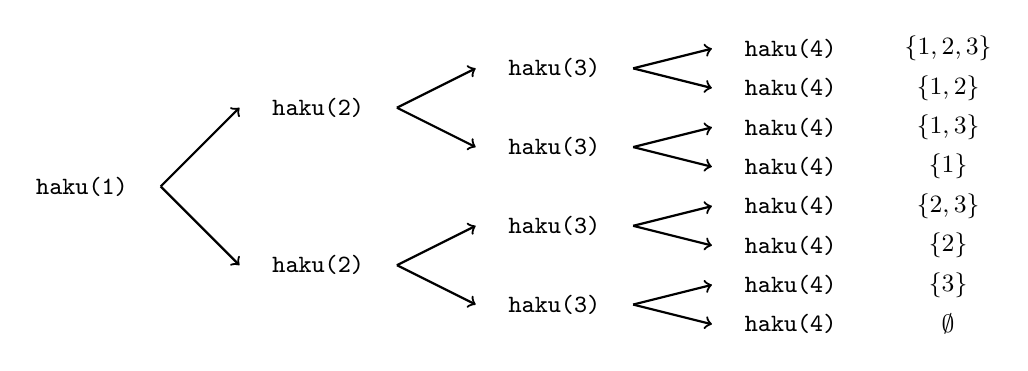
\begin{tikzpicture}[scale=0.5]
\small
\node at (0,0) {\texttt{haku(1)}};
\draw[thick,->] (2,0) -- (4,2);
\draw[thick,->] (2,0) -- (4,-2);
\node at (6.0,2) {\texttt{haku(2)}};
\node at (6.0,-2) {\texttt{haku(2)}};
\draw[thick,->] (8,2) -- (10,3);
\draw[thick,->] (8,2) -- (10,1);
\draw[thick,->] (8,-2) -- (10,-1);
\draw[thick,->] (8,-2) -- (10,-3);
\node at (12.0,3) {\texttt{haku(3)}};
\node at (12.0,1) {\texttt{haku(3)}};
\node at (12.0,-1) {\texttt{haku(3)}};
\node at (12.0,-3) {\texttt{haku(3)}};
\draw[thick,->] (14,3) -- (16,3.5);
\draw[thick,->] (14,3) -- (16,2.5);
\draw[thick,->] (14,1) -- (16,1.5);
\draw[thick,->] (14,1) -- (16,0.5);
\draw[thick,->] (14,-1) -- (16,-0.5);
\draw[thick,->] (14,-1) -- (16,-1.5);
\draw[thick,->] (14,-3) -- (16,-2.5);
\draw[thick,->] (14,-3) -- (16,-3.5);
\node at (18.0,3.5) {\texttt{haku(4)}};
\node at (18.0,2.5) {\texttt{haku(4)}};
\node at (18.0,1.5) {\texttt{haku(4)}};
\node at (18.0,0.5) {\texttt{haku(4)}};
\node at (18.0,-0.5) {\texttt{haku(4)}};
\node at (18.0,-1.5) {\texttt{haku(4)}};
\node at (18.0,-2.5) {\texttt{haku(4)}};
\node at (18.0,-3.5) {\texttt{haku(4)}};
\node at (22.0,3.5) {$\{1,2,3\}$};
\node at (22.0,2.5) {$\{1,2\}$};
\node at (22.0,1.5) {$\{1,3\}$};
\node at (22.0,0.5) {$\{1\}$};
\node at (22.0,-0.5) {$\{2,3\}$};
\node at (22.0,-1.5) {$\{2\}$};
\node at (22.0,-2.5) {$\{3\}$};
\node at (22.0,-3.5) {$\emptyset$};
\end{tikzpicture}
\caption{Osajoukkojen muodostaminen rekursiivisesti ($n=3$).}
\label{fig:osajou}
\end{figure}

\subsection{Permutaatioiden muodostaminen}

Tarkastellaan sitten toista ongelmaa, jossa haluammekin
käydä läpi lukujen $1,2,\dots,n$ \emph{permutaatiot}
eli kaikki mahdolliset tavat asettaa luvut johonkin järjestykseen.
Esimerkiksi tapauksessa $n=3$ lukujen permutaatiot ovat
$(1,2,3)$, $(1,3,2)$, $(2,1,3)$, $(2,3,1)$, $(3,1,2)$ ja $(3,2,1)$.

Myös permutaatioiden läpikäynti onnistuu kätevästi rekursiolla.
Ideana on, että valitsemme joka askeleella permutaatioon
jonkin luvun, joka ei vielä kuulu siihen.
Voimme toteuttaa haun näin:

\begin{code}
function haku(k)
    if k == n+1
        // käsittele permutaatio
    else
        for i = 1 to n
            if not mukana[i]
                mukana[i] = true
                permutaatio[k] = i
                haku(k+1)
                mukana[i] = false
\end{code}

Funktion parametri $k$ tarkoittaa, mihin permutaation kohtaan
valitsemme seuraavaksi luvun.
Haku alkaa, kun kutsumme funktiota parametrilla $k=1$.
Jos $k=n+1$, olemme saaneet permutaation valmiiksi
ja voimme käsitellä sen.
Muuten valitsemme permutaation kohtaan $k$ tulevan luvun
käymällä läpi silmukalla luvut $1 \dots n$.
Taulukko \texttt{mukana} kertoo, mitkä alkiot
ovat jo mukana permutaatiossa
Jos alkio $i$ ei ole vielä mukana, haaraudumme tapaukseen,
jossa valitsemme sen kohtaan $k$, ja jatkamme hakua kohtaan $k+1$.

Kun olemme saaneet permutaation valmiiksi,
voimme käsitellä sen esimerkiksi tulostamalla lukujen
järjestyksen näin:

\begin{code}
for i = 1 to n
    print(permutaatio[i])
\end{code}

Voimme valita permutaation ensimmäisen luvun $n$ tavalla,
toisen luvun $n-1$ tavalla,
kolmannen luvun $n-2$ tavalla, jne.,
minkä vuoksi luvuista $1,2,\dots,n$ voi muodostaa
kaikkiaan $n!$ permutaatiota.
Esimerkiksi tapauksessa $n=3$ permutaatioiden määrä on $3!=6$.

\subsection{Peruuttava haku}

Peruuttava haku on yleinen rekursiivinen menetelmä,
jota käyttäen voimme muodostaa järjestelmällisesti
kaikki ratkaisut annettuun ongelmaan.
Ideana on aloittaa tyhjästä ratkaisusta ja käydä
joka askeleella läpi rekursiivisesti kaikki mahdolliset tavat,
kuinka voimme laajentaa ratkaisua.

Peruuttava haku on raa'an voiman algoritmi,
ja voimme käyttää sitä vain silloin,
kun ratkaisujen määrä on niin pieni,
että ehdimme käydä läpi kaikki ratkaisut.
Kuitenkin jos voimme käyttää peruuttavaa hakua,
se on mainio tekniikka,
koska voimme olla varmoja, että oikein toteutettu
peruuttava haku löytää kaikki ratkaisut.

\begin{figure}
\center
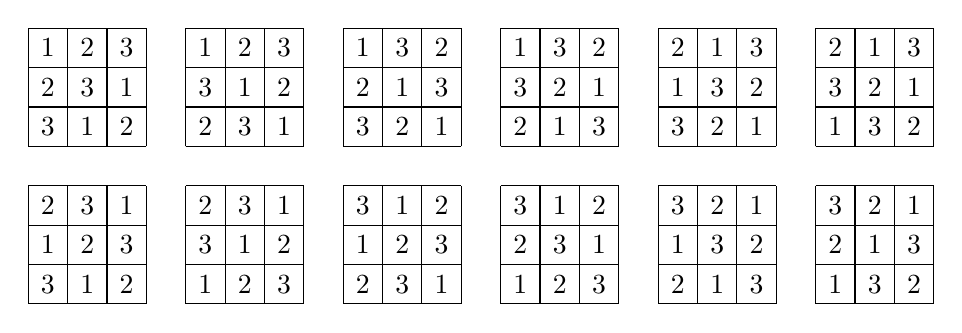
\begin{tikzpicture}[scale=0.5]
\newcommand\nelio[9]{
\draw (0,0) grid (3,3);
\foreach \x/\y/\v in {0/0/#1,1/0/#2,2/0/#3,0/1/#4,1/1/#5,2/1/#6,0/2/#7,1/2/#8,2/2/#9} \node at (0.5+\x,2.5-\y) {\v};
}
\begin{scope}
\nelio{1}{2}{3}{2}{3}{1}{3}{1}{2}
\end{scope}
\begin{scope}[xshift=4cm]
\nelio{1}{2}{3}{3}{1}{2}{2}{3}{1}
\end{scope}
\begin{scope}[xshift=8cm]
\nelio{1}{3}{2}{2}{1}{3}{3}{2}{1}
\end{scope}
\begin{scope}[xshift=12cm]
\nelio{1}{3}{2}{3}{2}{1}{2}{1}{3}
\end{scope}
\begin{scope}[xshift=16cm]
\nelio{2}{1}{3}{1}{3}{2}{3}{2}{1}
\end{scope}
\begin{scope}[xshift=20cm]
\nelio{2}{1}{3}{3}{2}{1}{1}{3}{2}
\end{scope}
\begin{scope}[yshift=-4cm]
\nelio{2}{3}{1}{1}{2}{3}{3}{1}{2}
\end{scope}
\begin{scope}[yshift=-4cm,xshift=4cm]
\nelio{2}{3}{1}{3}{1}{2}{1}{2}{3}
\end{scope}
\begin{scope}[yshift=-4cm,xshift=8cm]
\nelio{3}{1}{2}{1}{2}{3}{2}{3}{1}
\end{scope}
\begin{scope}[yshift=-4cm,xshift=12cm]
\nelio{3}{1}{2}{2}{3}{1}{1}{2}{3}
\end{scope}
\begin{scope}[yshift=-4cm,xshift=16cm]
\nelio{3}{2}{1}{1}{3}{2}{2}{1}{3}
\end{scope}
\begin{scope}[yshift=-4cm,xshift=20cm]
\nelio{3}{2}{1}{2}{1}{3}{1}{3}{2}
\end{scope}
\end{tikzpicture}
\caption{Kaikki 12 latinalaista neliötä kokoa $3 \times 3$.}
\label{fig:latnel}
\end{figure}

Tarkastellaan esimerkkinä tehtävää, jossa haluamme käydä läpi
kaikki kokoa $n \times n$ olevat \emph{latinalaiset neliöt}
eli ruudukot, joissa kullakin vaaka- ja pystyrivillä
esiintyy tarkalleen kerran jokainen luku $1,2,\dots,n$.
Kyseessä on siis yksinkertaistus tutusta sudoku-tehtävästä.
Esimerkiksi kuva \ref{fig:latnel} näyttää kaikki 12 latinalaista neliötä kokoa $3 \times 3$.

Toteutamme peruuttavan haun niin, että valitsemme joka askeleella
ruudukon kohtaan $(y,x)$ tulevan luvun.
Numeroimme ruudukon vaaka- ja pystyrivit kokonaisluvuin $1,2,\dots,n$.
Aloitamme haun ruudukon vasemmasta yläkul\-masta ja etenemme
rivi kerrallaan alaspäin.
Seuraava rekursiivinen algoritmi toteuttaa haun,
kun sitä kutsutaan parametreilla $(1,1)$:

\begin{code}
function haku(y,x)
    if y == n+1
        // käsittele ratkaisu
    else if x == n+1
        haku(y+1,1)
    else
        for i = 1 to n
            if not vaaka[y][i] and not pysty[x][i]
                vaaka[y][i] = pysty[x][i] = true
                nelio[y][x] = i
                haku(y,x+1)
                vaaka[y][i] = pysty[x][i] = false
\end{code}

Algoritmin alussa on kaksi erikoistapausta:
jos $y=n+1$, olemme saaneet muodostettua
yhden latinalaisen neliön.
Jos taas $x=n+1$, olemme saaneet jonkin vaakarivin
valmiiksi ja alamme muodostaa seuraavaa vaakariviä.
Muuten kyseessä on perustapaus, jossa haluamme
valita kohtaan $(y,x)$ tulevan luvun.
Käymme läpi kaikki mahdolliset tavat for-silmukalla,
jossa $i$ on valittava luku.
Koska jokainen luku saa esiintyä vain kerran kullakin
vaaka- ja pystyrivillä, käytämme kahta aputaulukkoa:
$\texttt{vaaka}[y][i]$ kertoo, onko vaakarivillä $y$
jo lukua $i$, ja vastaavasti $\texttt{pysty}[x][i]$ kertoo,
onko pystyrivillä $x$ jo lukua $i$.
Jos voimme sijoittaa luvun $i$ kohtaan $(y,x)$,
merkitsemme tämän taulukkoon $\texttt{nelio}[y][x]$
ja lisäksi päivitämme taulukoita $\texttt{vaaka}$ ja $\texttt{pysty}$.
Sitten jatkamme hakua rekursiivisesti seuraavaan
oikealla olevaan ruutuun.

\begin{table}
\center
\begin{tabular}{rr}
ruudukon koko $n$ & neliöiden määrä \\
\hline
1 & 1 \\
2 & 2 \\
3 & 12 \\
4 & 576 \\
5 & 161280 \\
6 & 812851200 \\
\end{tabular}
\caption{Latinalaisten neliöiden määrät, kun $n=1,2,\dots,6$.}
\label{tab:latnel}
\end{table}

Kun olemme saaneet muodostettua latinalaisen neliön, voimme
tulostaa sen sisällön taulukon \texttt{nelio} perusteella
tai vain laskea, montako neliötä on olemassa.
Taulukko \ref{tab:latnel} sisältää latinalaisten neliöiden
määrät tapauksissa $n=1,2,\dots,6$, jotka pystymme laskemaan nopeasti.
Suuremmilla $n$:n arvoilla haku alkaa kestää liian kauan
ja meidän tulisi keksiä keino tehostaa hakua,
jos haluaisimme laskea neliöiden määriä suuremmissa tapauksissa.

\section{Matemaattinen tausta}

Tietorakenteiden ja algoritmien teoria perustuu matematiikkaan,
ja käym\-me kirjassa pikkuhiljaa läpi tarvittavia tietoja.
Seuraavassa on joitakin merkintöjä ja käsitteitä, joista on hyötyä
useassa kirjan kohdassa.

\subsection{Summakaavat}

Voimme laskea lukujen $1,2,\dots,n$ summan kaavalla
\[1+2+\dots+n = \frac{n(n+1)}{2}.\]
Esimerkiksi
\[1+2+3+4+5 = \frac{5 \cdot 6}{2}=15.\]
Kaavan voi ymmärtää niin, että laskemme yhteen $n$ lukua,
joiden suuruus on \emph{keskimäärin} $(n+1)/2$.

Toinen hyödyllinen kaava on
\[2^0+2^1+\dots+2^n = 2^{n+1}-1.\]
Esimerkiksi
\[1+2+4+8+16=32-1.\]
Tässä voimme ajatella, että aloitamme luvusta $2^n$
ja lisäämme siihen aina puolet pienemmän luvun lukuun $1$ asti.
Tämän seurauksena pääsemme yhtä vaille lukuun $2^{n+1}$ asti.

Esitämme joskus summia merkinnän $\sum$ avulla.
Siinä on ideana antaa muuttujan ala- ja yläraja sekä
joka askeleella summaan lisättävä arvo.
Esimerkiksi voimme merkitä
\[1^2 + 2^2 + \dots + n^2 = \sum_{i=1}^n i^2.\]

Tämä merkintä on itse asiassa hyvin lähellä ohjelmoinnin
for-silmukkaa, koska seuraava koodi ajaa saman asian:

\begin{code}
summa = 0
for i = 1 to n
    summa += i*i
\end{code}

\subsection{Logaritmit}

Logaritmin määritelmän mukaan $\log_b n =x$
tarkalleen silloin kun $b^x=n$.
Esimerkiksi $\log_2 32=5$, koska $2^5=32$.

Algoritmiikassa logaritmin kantaluku $b$ on usein 2,
ja voimme ajatella, että logaritmi kertoo, montako kertaa
meidän täytyy \emph{puolittaa} luku $n$, ennen kuin pääsemme lukuun 1.
Esimerkiksi $\log_2 32 =5$, koska tarvitsemme 5 puolitusta:
\[32 \rightarrow 16 \rightarrow 8 \rightarrow 4 \rightarrow 2 \rightarrow 1\]
Tässä kirjassa oletamme, että logaritmin kantaluku on 2,
jos ei ole toisin mainittu,
eli voimme kirjoittaa lyhyesti $\log 32 = 5$.

Logaritmeille pätee kaavat
\[\log_b(x \cdot y) = \log_b(x)+\log_b(y)\]
ja
\[\log_b(x / y) = \log_b(x)-\log_b(y).\]
Ylemmästä kaavasta seuraa myös
\[\log_b(x^k) = k \log_b(x).\]
Lisäksi voimme vaihtaa logaritmin kantalukua kaavalla
\[\log_u(x) = \frac{\log_b(x)}{\log_b(u)}.\]
